\NoBgThispage
\chapter{Localization on HD maps}
The purpose of this chapter is to provide an overview, before delving into the specifics, to first understand what High Definition (HD) maps are and their significance in the field of autonomous driving.

\section{Autonomous Driving}
The concept of autonomous driving has evolved from a theoretical idea to a rapidly advancing field with profound technological, societal, and legal implications. Autonomous vehicles (AVs) hold the potential to revolutionize transportation by improving safety, reducing congestion, and enhancing mobility \cite{9695620}. The technological backbone of this transformation involves advanced sensors, machine learning algorithms, vehicle-to-everything (V2X) communication, and real-time decision-making algorithms. At the core of understanding the complexity and potential of autonomous vehicles lies the classification system developed by the Society of Automotive Engineers (SAE)\footnote{SAE is the society which decided to declare what autonomous driving is and how has to be categorized in order to be precise and compliant.} \cite{sae2021}, which defines the various stages of vehicle automation.

The SAE International established a six-tier classification system in 2014, which was refined in subsequent years, to standardize the levels of driving automation across the industry. The levels range from Level 0, where no automation exists, to Level 5, representing full automation. Each level represents a step toward the ultimate goal of a fully autonomous vehicle, and these levels are essential in understanding the current and future development of AV technology \cite{9881892}.

\begin{figure}
    \centering
    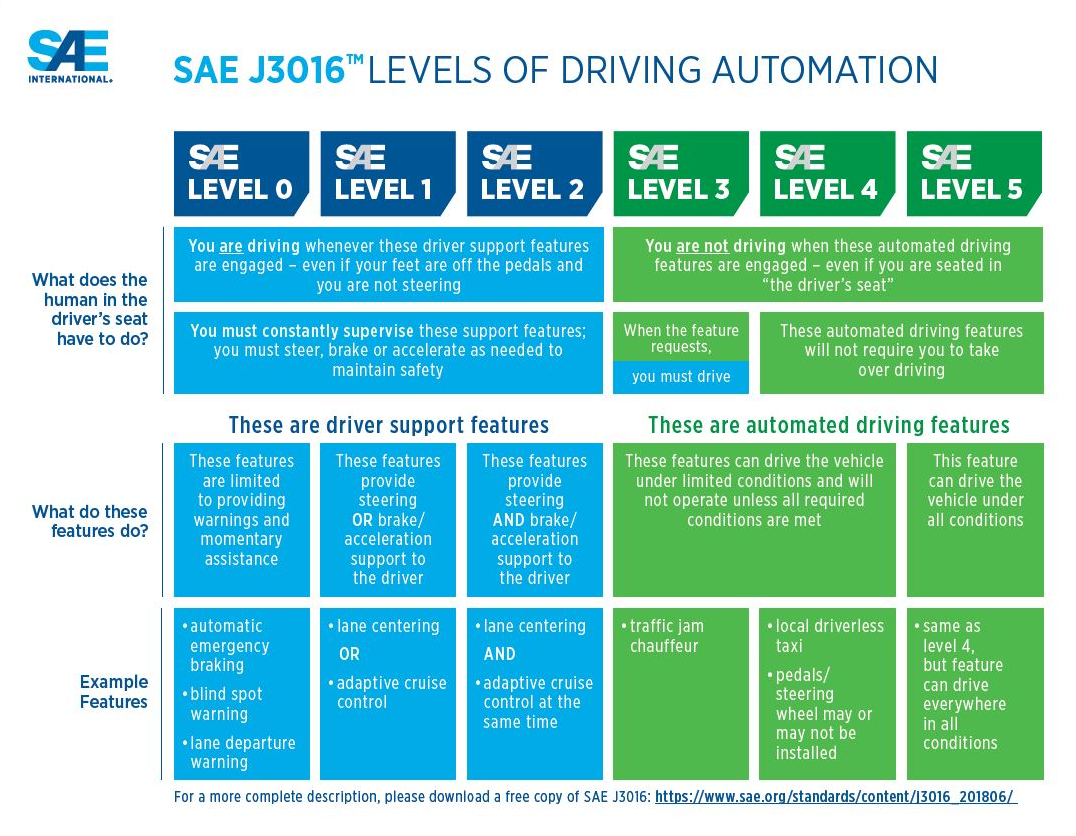
\includegraphics[width=1\linewidth]{LateX/figs/ca3qj6bg.png}
    \caption{SAE J3016 levels of driving automation.}
    \label{fig:sae_levels_of_automation}
\end{figure}

\begin{itemize}
    \item Level 0: No Automation – At this level, the human driver is fully responsible for all tasks, though the vehicle may provide warnings or momentary assistance, such as automatic emergency braking (SAE J3016).
    \item Level 1: Driver Assistance – Vehicles at this level are equipped with systems like adaptive cruise control, where the driver remains in control but can benefit from limited automated assistance in specific scenarios.
    \item Level 2: Partial Automation – Level 2 vehicles can control both steering and acceleration/deceleration under certain conditions, but the human driver must remain attentive and ready to take over at any time.
    \item Level 3: Conditional Automation – At this level, the vehicle can manage most driving tasks, but the driver must be available to overtake when requested by the system. This level marks a significant milestone as the vehicle can make decisions autonomously under specific circumstances.
    \item Level 4: High Automation – Vehicles at Level 4 can operate without human intervention in certain conditions or geographic areas. However, a driver may still be required for situations outside the vehicle's operational design domain.
    \item Level 5: Full Automation – At the highest level, the vehicle can operate autonomously in all conditions and environments, without any need for human input. This level predicts a future where transportation no longer relies on human drivers.
\end{itemize}

The progression through these levels is not just a technical challenge but involves addressing ethical, regulatory, and safety concerns. Autonomous driving technology is a complex field that incorporates artificial intelligence, sensor fusion, human-machine interaction, and cybersecurity.

% ----------------------------------------------------------------------------------------
\section{HD Maps}
% ----------------------------------------------------------------------------------------


Before delving into the specifics, it is crucial to first understand what High Definition (HD) maps are and their significance in the field of autonomous driving.

High-definition (HD) semantic maps are an essential module for autonomous driving. Traditional pipelines to construct
such HD semantic maps involve capturing point clouds beforehand, building globally-consistent maps using SLAM,
and annotating semantics in the maps. 

https://arxiv.org/pdf/2107.06307 -> questo paper mi sembra abbastanza simile a quello che prevede la RTMG, si tratta di qualcosa di simile che va a ricreare una local HD maps dai dati proveniente dal sensore senza andare a considerare una vera mappa HD che sarebbe molto difficile e costosa da mantenere e soprattutto da mentere aggiornata nel tempo considerando che la strada è soggetta a cambiamenti quotidiani che vanno dai cantieri, ai lavori in corso, alla costruzione di nuove ciclabili, alla viabilità modificata per altre motivazioni ecc ecc


This kind of maps can be distinguished by their extremely high precision, often at the centimeter level. According to Geospatial World specifically have extremely high precision at centimeter-level.

https://www.geospatialworld.net/article/hd-maps-autonomous-vehicles/

Self-driving vehicles require precise localization to navigate safely, especially under challenging conditions such as poor weather. 
Despite the high precision of HD maps, their utility is significantly diminished without accurate localization. Thus, while these maps provide crucial data, the ability to accurately determine a vehicle's position is fundamental to leveraging the full potential of HD maps in autonomous driving.

\begin{figure}
    \centering
    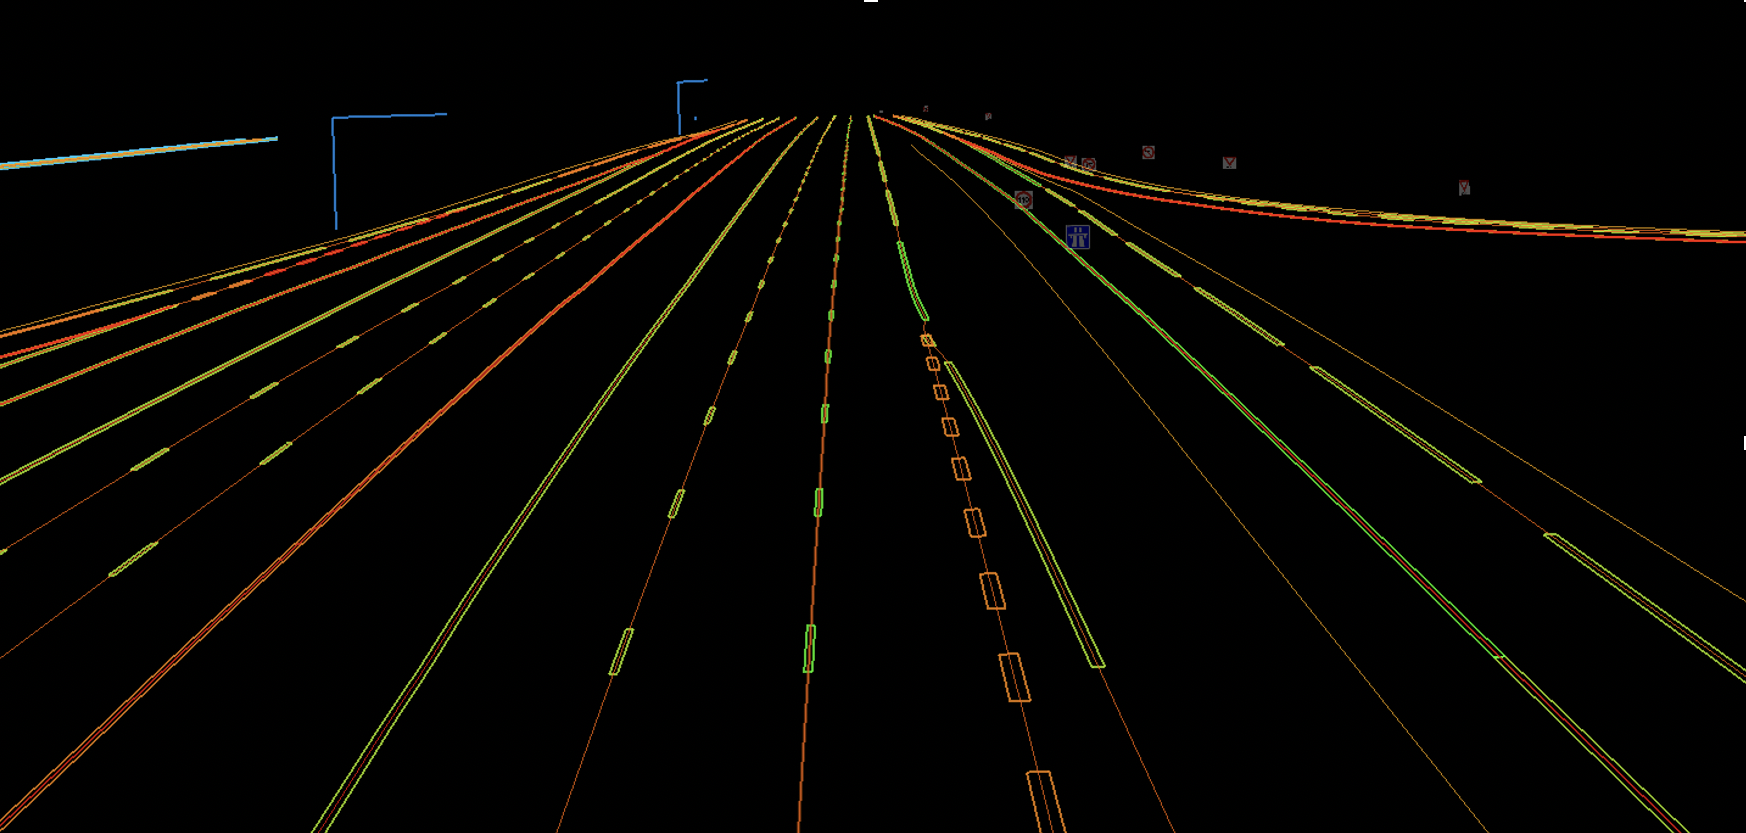
\includegraphics[width=1\linewidth]{LateX/figs/Screenshot-2021-07-16-at-17.00.59-e1626451336528.png}
    \caption{Enter Caption}
    \label{fig:enter-label}   
\end{figure}


\begin{figure}
    \centering
    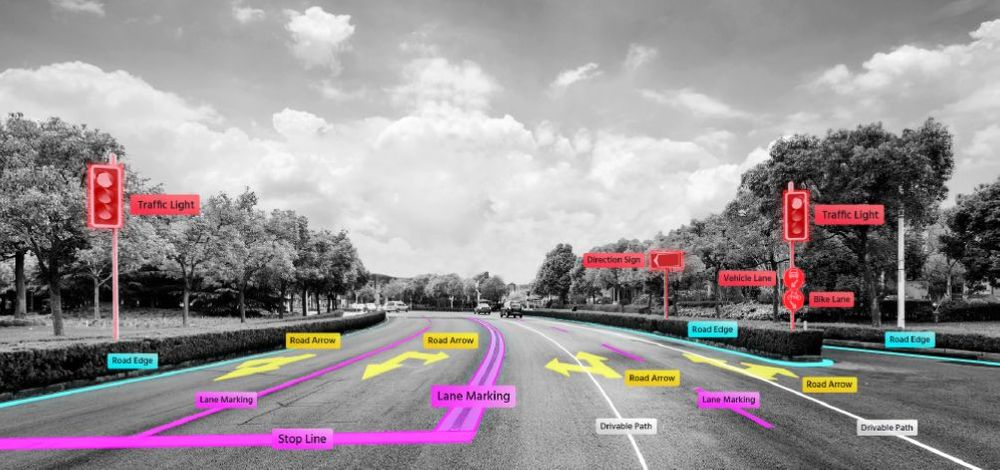
\includegraphics[width=1\linewidth]{LateX/figs/35493487c9d025c81f4e9ed21722d458_1612794598859.jpg}
    \caption{Enter Caption}
    \label{fig:enter-label}
\end{figure}


www.autonomousvehicleinternational.com/features/the-road-to-everywhere-are-hd-maps-for-autonomous-driving-sustainable.html 

https://www.sciencedirect.com/science/article/pii/S2667325824000268

\subsection{HD maps}
Before going into details it is better to starting analyzing what HD maps are and which is their importance in the autonomous driving field. 

"The maps that are particularly built for self-driving purposes are usually called High Definition Maps or HD Maps. These maps specifically have extremely high precision at centimeter-level." (questa è una citazione presa dal sito https://www.geospatialworld.net/article/hd-maps-autonomous-vehicles/)

(ecco qui un'altra fonte da cui prendere un po' di informazioni)
https://medium.com/wovenplanetlevel5/https-medium-com-lyftlevel5-rethinking-maps-for-self-driving-a147c24758d6

A self-driving car needs to know where it is at all times, especially in poor weather. The TomTom HD Map helps vehicles know their exact location on the road – down to the centimeter. TomTom RoadDNA works with any sensor layout to enhance positioning with localization map layers that contain multiple sets of format-friendly data.

https://www.tomtom.com/products/hd-map/

(magari citare qualcosa di openstreet maps e di come le mappe create dagli utenti possano essere viste come mappe HD)
OpenStreetMap is built by a community of mappers that contribute and maintain data about roads, trails, cafés, railway stations, and much more, all over the world.

Local Knowledge
OpenStreetMap emphasizes local knowledge. Contributors use aerial imagery, GPS devices, and low-tech field maps to verify that OSM is accurate and up to date.

Community Driven
OpenStreetMap's community is diverse, passionate, and growing every day. Our contributors include enthusiast mappers, GIS professionals, engineers running the OSM servers, humanitarians mapping disaster-affected areas, and many more. To learn more about the community, see the OpenStreetMap Blog, user diaries, community blogs, and the OSM Foundation website.

Open Data
OpenStreetMap is open data: you are free to use it for any purpose as long as you credit OpenStreetMap and its contributors. If you alter or build upon the data in certain ways, you may distribute the result only under the same licence. See the Copyright and License page for details.

Quindi parlare di quanto siamo importanti in quanto a precision ecc, citare quelle che sono le più utilizzate, per poi arrivare a dire che sono completamente inutili se non si è in grado di localizzarcisi sopra. 

(da questo sito prendere le immagini per questa parte, sembra fatto bene e le immagini sono di qualità)
https://www.autonomousvehicleinternational.com/features/the-road-to-everywhere-are-hd-maps-for-autonomous-driving-sustainable.html












High-definition maps for self-driving cars usually include map elements such as road shape, road marking, traffic signs, and barriers.[4][10] Maintaining high accuracy is one of the biggest challenges in building HD maps of real-world roads. With regard to accuracy, there are two main focus points that determine the quality of an HD map:

Global accuracy (positioning of a feature on the surface of the Earth)
Local accuracy (positioning of a feature in relation to road elements around it).
In areas with good GPS reception it is possible to achieve a global accuracy of less than 3 cm deviation using satellite signals and correction data from base stations.

In GPS-denied areas, however, inaccuracy rises with distance traveled through the area, being largest in its middle. This means that the maximum GPS error can be expressed as a percentage of the distance traveled through a GPS-denied area: this value is less than 0.5%.[11]

https://en.wikipedia.org/wiki/High-definition_map





What are HD maps?
Sometimes called by their full name of high-definition maps, HD maps have many more details than traditional varieties do. They’re typically shown at the centimeter scale. Instead of merely indicating things like the locations of particular places or the distance between two destinations, HD maps feature information about lane placement, road boundaries, the severity of curves, the gradient of the road surface, and more.

Providing detail to this extent is crucial because so much inconsistency exists between roads. For example, bike lanes can be different widths depending on if they’re marked or unmarked. Plus, some city planners may choose to make those lanes substantially wider than the minimum in places with exceptionally heavy traffic.

If an autonomous car’s technology makes the vehicle maneuver as if all bike lanes are a uniform width, riders could be at risk for collisions. Bike lanes are just one example.

Traditional maps are for humans to read. People can use things like experience and depth perception when constantly assessing their environment and ensuring they don’t run off the road or veer into another lane. Since autonomous cars don’t have the same abilities as humans, they need maps that support what they can do. HD maps provide information that helps driverless vehicles move from one location to another without making errors.

How are HD maps structured?
HD maps have information presented in layers. This arrangement works well, considering the amount of data it must contain. As of now, there is no standardization between the businesses making 3D maps. The data in each layer varies depending on the company that produces the map.

https://iot.eetimes.com/what-are-hd-maps-and-how-will-they-get-us-closer-to-autonomous-cars/



From ADAS slides:
Hd maps can be defines as a 3d reconstruction of the road environment. They can be used to manage the behavioral planning of an autonomous vehicle. 
HD Maps should include:
- connection between lanes (even implicit)
- lane markings, curbs, traffic signs, pedestrian crossings, and so on 
- traffic lights (coupled with lanes)  
- altitude 

GUARDARE ANCHE LA PAGINA DI HERE IN CUI VENGONO DESCRITTE LE MAPPE HD, hd road, hd lane and hd localization 
GUARDARE ANCHE SUL SITO DI TOMTOM la parte destinata alle hd maps 
TROVARE ANCHE UN'IMMAGINE SIMILE A QUELLA CHE C'È NELLE SLIDE DI ADAS, QUELLA È SICURAMENTE GIUSTA 



An HD Map is not just a navigation map
but a powerful “sensor” that provides detailed information around and further around the
corner to support ego vehicle perception once it is localised in the map (EDMap, 2004)
\textit{Fonte: EDMap. (2004). Enhanced Digital Mapping Project Final Report. Submitted to the United States Department
of Transportation, Federal Highway Administration and National Highway Traffic and Safety Administration.
https://goo.gl/SPF7h8. Accessed on 5 June 2019.}


The different levels of automated driving tasks require that the world is modelled at
different levels of details. HD Maps are not only the storage for globally referenced road
networks and lane level details but also provide unique landmarks or the whole appearance
of the surrounding environment to aid ego vehicle localisation. Both HD Maps and the
pose of the ego vehicle are inputs to the perception module for world modelling, from
which the planning and control module deduces actions and plans. On the other hand, the
world model can also be fed back to make HD Maps up-to-date.

GUARDARE ANCHE NELLA BIBLIOGRAFIA DELL'ARTICOLO DI CAMBRIDGE PERCHÈ CI SONO DAVVERO MOLTE COSE INTERESSANTI

https://www.cambridge.org/core/journals/journal-of-navigation/article/high-definition-map-for-automated-driving-overview-and-analysis/7FFB4F68B9C27F4312AF8DCD553205FE



% ----------------------------------------------------------------------------------------
\section{Localization on HD maps}
% ----------------------------------------------------------------------------------------

si potrebbe parlare delle varie tecniche e dell'importanza di localizzarvicisi sopra

questa è una parte che può essere scritta meglio e che può essere analizzata: Una mappa può essere considerata come un grafo orientato 

Gli archi dovranno essere pesati, in base alle informazioni che vogliamo tenere in conto. 

Dobbiamo sempre essere geo-localizzati sia nel nodo sia nel ramo.

---


https://ieeexplore.ieee.org/stamp/stamp.jsp?tp=&arnumber=10670300
questo è un paper che si potrebbe citare e che trovo utile 


https://journals.sagepub.com/eprint/VUKQIDNVMJRXZADHANNG/full
qui si potrebbe dire che la mapppa hd è sia utile nel contesto di localizzarcisi sopra, sia può essere utile per il contrario, ovvero come sensore di localizzazione e quindi capire dalla mappa la posizione del veicolo. 


https://journals.sagepub.com/eprint/VUKQIDNVMJRXZADHANNG/full
Anche qui c'è un elenco di approcci che si possono utilizzare per andare a localizzarsi all'interno di una mappa HD.

essenzialmente c'è l'approccio del solo gps e poi quello di sfruttare tutti i sensori. ciò che è diverso nel mio case study è il fatto che questo ultimo procedimento venga fatto direttamente con una rete senza passare da nessun problema di ottimizzazione.



The purpose of this chapter is to provide an overview of the current state of the art in the field of localization on High Definition (HD) maps, which is a critical aspect of autonomous driving technology. By reviewing relevant literature and discussing key concepts, this chapter aims to outline the fundamental role of HD maps in achieving precise vehicle localization, explore the sensor suite necessary for localization, and examine the various methods and challenges associated with localization on HD maps.

\section{HD Maps: Definition and Importance}
High Definition (HD) maps are a foundational component in the navigation systems of autonomous vehicles. Unlike traditional maps designed for human use, HD maps contain a wealth of detailed information, including road geometry, lane markings, traffic signs, and other infrastructure data, all presented at a centimeter-level accuracy. These maps are indispensable for autonomous driving, where even slight errors in localization can lead to critical failures. The precision of HD maps allows autonomous vehicles to navigate complex environments with a high degree of safety, especially in scenarios where sensor data alone may be insufficient, such as during poor weather conditions.

\begin{figure}
    \centering
    \includegraphics[width=1\linewidth]{LateX//figs/CAP1_MERGE_HD_MAP.pdf}
    \caption{Enter Caption}
    \label{fig:enter-label}
\end{figure}

As outlined by sources like Geospatial World \cite{geospatialworld_hd_maps}, HD maps feature extraordinarily high precision, often to within a few centimeters. These maps are not static representations but dynamic systems continuously updated to ensure the most accurate depiction of the surrounding environment. They offer a layer of data that enhances the decision-making processes of self-driving cars by providing critical information on road attributes such as lane width, road curvature, altitude, and traffic rules. This wealth of data ensures that the vehicle can make informed decisions and maintain safe driving behavior, particularly in complex urban scenarios.

\subsection{The Structure of HD Maps}
HD maps are structured in multiple layers to efficiently manage the large volumes of data required for autonomous navigation. These layers include everything from the physical layout of roads and lanes to more abstract information such as traffic flow and regulatory signs. However, the lack of industry standardization in HD map formats means that different companies may design their maps using different data models, although the core elements remain largely the same.
Key elements included in HD maps typically are:

\begin{itemize}
    \item Road geometry and lane structure: Including lane markings, road curvature, and road boundaries.
    \item Environmental features: Traffic signs, pedestrian crossings, and curbs.
    \item Dynamic information: Data related to traffic flow and temporary obstructions.
\end{itemize}

One significant advantage of HD maps is their ability to serve as an additional sensor for autonomous vehicles, as described by the Enhanced Digital Mapping Project (EDMap) \cite{edmap_2004} . In this context, the HD map acts as a reliable source of information that can supplement real-time sensor data, allowing vehicles to perceive their surroundings more accurately even in situations where sensors like cameras and LiDAR may be compromised by environmental factors.


ATTENZIONE %%%TODO


In the realm of automated driving systems, high-definition (HD) maps are integral due to their comprehensive detailing of road features. Lane-level geometry, as depicted in HD maps, plays a pivotal role in enhancing lateral and longitudinal control by providing precise information about the road's curvature and slope. Lane-level speed limits within these maps ensure that vehicles can regulate their speed in accordance with posted limits, contributing to smoother and safer driving. Lane markings are detailed in HD maps to assist vehicles in adhering to traffic rules and staying within their designated lanes. The inclusion of traffic light data in these maps allows for the accurate timing of stops and the safe navigation of intersections and highway ramps. Road borders and guardrails are mapped to support proper lateral positioning and to define the operational design domain, which is crucial for maintaining vehicle stability. Lane connectivity information enables vehicles to determine and follow a safe and efficient path, facilitating seamless transitions between road segments. Finally, comprehensive on/off ramp coverage in HD maps ensures that vehicles can merge onto highways and perform automated lane changes with confidence, promoting a smooth and comfortable driving experience.


\subsection{Localization on HD Maps}
The value of HD maps is intrinsically linked to their use in vehicle localization. Localization refers to the process by which a vehicle determines its precise position on the map. Without accurate localization, even the most detailed HD map would be of little practical use. Localization involves the integration of data from various sensors, such as GPS, LiDAR, cameras, and inertial measurement units (IMUs), with the information contained in HD maps.

There are several approaches to localization on HD maps, each with its strengths and limitations. These methods generally fall into two categories: map-based localization and sensor-based localization.

Map-based Localization
In map-based localization, the vehicle continuously matches its sensor data with the pre-existing data in the HD map. For example, LiDAR point clouds can be compared against the road geometry and landmarks in the HD map, allowing the vehicle to determine its position with a high degree of accuracy. This method is particularly effective in urban environments where detailed HD maps contain abundant landmarks that can be used for precise positioning.

However, one of the primary limitations of map-based localization is its dependency on the quality of the HD map. If the map is outdated or incomplete, localization accuracy can be severely compromised. Moreover, areas with poor GPS reception, such as tunnels or dense urban canyons, pose additional challenges, although modern systems employ techniques like sensor fusion to mitigate these issues.

Sensor-based Localization
Sensor-based localization relies on the vehicle’s onboard sensors to determine its position relative to the environment, which is then corrected or enhanced by data from the HD map. For instance, systems like TomTom’s RoadDNA use sensors to capture the road's detailed surface structure, which is then compared with the map data to enhance localization accuracy .

One approach is simultaneous localization and mapping (SLAM), where the vehicle not only localizes itself but also constructs or updates the map in real-time. This method is particularly valuable in environments where HD maps may be incomplete or unavailable. However, SLAM systems face challenges in ensuring global consistency, especially over long distances, where drift and inaccuracies may accumulate.

Challenges and Future Directions
Despite significant advancements, there are several challenges to achieving robust and reliable localization on HD maps. First, maintaining the accuracy of HD maps in dynamic environments is an ongoing challenge. Road conditions can change due to construction, accidents, or temporary obstacles, and HD maps need to be updated frequently to remain useful. The real-time updating of maps is an area of active research and development, with companies exploring crowd-sourced map updates and the use of connected vehicle fleets to maintain map accuracy.

Additionally, the fusion of multiple sensor data streams—such as GPS, LiDAR, and cameras—with HD maps remains a complex task. Sensor inaccuracies, environmental noise, and occlusions can all introduce errors that affect localization performance. As a result, one of the key areas of ongoing research is improving the algorithms that integrate these diverse data sources, enabling more robust and reliable localization even in challenging conditions like GPS-denied areas.

Another significant challenge is the scalability of HD maps. Creating and maintaining these highly detailed maps across large geographical areas is resource-intensive. Solutions such as user-generated maps, like those provided by OpenStreetMap, offer potential alternatives by enabling communities to contribute to map development and maintenance . However, achieving the precision required for autonomous driving remains a challenge in these open-source systems.

Conclusion
HD maps play an indispensable role in the safe and reliable operation of autonomous vehicles. Their high level of detail, combined with precise localization techniques, allows vehicles to navigate complex environments with confidence. However, the integration of HD maps with sensor data to achieve accurate localization is not without its challenges. Maintaining map accuracy, improving sensor fusion algorithms, and addressing the scalability of HD map systems are all areas that will require further research and development. As the field of autonomous driving continues to evolve, HD maps and localization techniques will remain central to overcoming the technical hurdles that lie ahead.







ALTRE FONTI 
https://www.tomtom.com/products/hd-map/

UNA LISTA DI LINK DOVE SI POSSONO TROVARE UN PO' DI IMMAGINI:

https://arstechnica.com/cars/2017/03/the-most-detailed-maps-of-the-world-will-be-for-cars-not-humans/

https://www.autonomousvehicleinternational.com/features/the-road-to-everywhere-are-hd-maps-for-autonomous-driving-sustainable.html

https://i.ytimg.com/vi/wKoV_fsP4_s/maxresdefault.jpg (Atlatec)

https://techcrunch.com/wp-content/uploads/2022/03/DRIVE-Map-2.jpg

https://s1.cdn.autoevolution.com/images/news-gallery-860x/how-mobileye-might-beat-tesla-at-its-own-self-driving-game-thumbnail_1.jpg

https://www.cambridge.org/core/services/aop-cambridge-core/content/view/7FFB4F68B9C27F4312AF8DCD553205FE/S0373463319000638a.pdf/high-definition-map-for-automated-driving-overview-and-analysis.pdf

DEVO assolutamente buttare giù un indice in modo da poter sapere hce cosa devo fare e quello che devo sdcrivere nelle varie strutture. a quel punto, mi ripulisco il modello dallo shcifo che c'è della tesi triennale e inizio a pensare a che cosa devo metterci per quanto riguarda questa. avrò già pensato a quelli che sono i nuovi capitoli ecc. 
devo anche iniziare a capire come e che cosa ho intezione di fare con le immagini, devo effettivamente fare qualcosa di sostenibile, altrimenti non ha senso. non posso pensare di ricopiarle tutte.
devo anche gestire in modo furbo il materiale, creando delle cartelle che sono effettivamente sempre sincronizzate in modo da evitare qualsiasi rischio che invece mi ero preso con la triennale mantenendo tutto in locale, tant'è che avendo formattato il computer ho perso praticamente tutto.
Di tutti i link che mi sono preparato devo anche sbatterli nella bibliografia in modo da avere già tutto e non stare a pensare anche a quello.


una brevissima introduzione sull'autonomous driving e sui livelli SAE in modo da poterli utilizzare forse la farei. ci vuole anche poco a farla e si trovano immagini carine 
https://themvp.com/blog/levels-of-automated-driving/
qui c'è un'immagine carina 



ALTRA FONTE PER UN'IMMAGINE CARINA 
https://arxiv.org/pdf/2107.06307
@misc{li2022hdmapnetonlinehdmap,
      title={HDMapNet: An Online HD Map Construction and Evaluation Framework}, 
      author={Qi Li and Yue Wang and Yilun Wang and Hang Zhao},
      year={2022},
      eprint={2107.06307},
      archivePrefix={arXiv},
      primaryClass={cs.CV},
      url={https://arxiv.org/abs/2107.06307}, 
}